\documentclass[a4paper]{article}%formato de plantilla%
\usepackage[utf8]{inputenc}
\usepackage[spanish]{babel}
\usepackage[margin=2cm, top=2cm, includefoot]{geometry}
\usepackage{graphicx} %para la insercion de imagenes 
\usepackage[table,xcdraw]{xcolor} % Para la deteccion de colores
\usepackage[most]{tcolorbox} % Para la insercion de cuadores en la portada
\usepackage{fancyhdr} %Definir el estilo de la pagina 
\usepackage[hidelinks]{hyperref} % Gestion de hipervinculos
\usepackage{parskip} %Arreglo d la tabulacion en el documento
\usepackage[figurename=Figura]{caption} % Cambiar el nombre del caption de las fotos
\usepackage{smartdiagram} % Para la insercion de diagramas 


%Declaracion de colores 
\definecolor{greenPortada}{HTML}{69A84F}

%Declaracion de variables%
\newcommand{\logoPortada}{try_hack_me.png}
\newcommand{\machineName}{Ice} %nombre de la maquina
\newcommand{\logoMachine}{ice_logo.png} % logo de la maquina
\newcommand{\startDate}{5 de Mayo del 2020}

% Adicionales 
\addto\captionsspanish{\renewcommand{\contentsname}{Indice}} % Cambio del formato del Indice
\setlength{\headheight}{40.2pt}
\pagestyle{fancy}
\fancyhf{}
\lhead{\includegraphics[width=2.5cm]{\logoPortada}}\rhead{\includegraphics[height=1.5cm]{\logoMachine}}
\renewcommand{\headrulewidth}{3pt}
\renewcommand{\headrule}{\hbox to\headwidth{\color{greenPortada}\leaders\hrule height \headrulewidth\hfill}}


%Comienzo del documento 
\begin{document}
	\cfoot{\thepage}
	%Creacion de portada 
	\begin{titlepage}
	\centering
	\includegraphics[width=0.5\textwidth]{\logoPortada}\par\vspace{1cm}
	{\scshape\LARGE \textbf{Informe Tecnico}\par }
	\vspace{0.2cm}
	{\Huge\bfseries\textcolor{greenPortada}{Room \machineName}\par}
	\vfill\vfill
	\includegraphics[width=\textwidth,height=8cm,keepaspectratio]{\logoMachine}\par\vspace{1cm}
	\vfill
	\begin{tcolorbox}[colback=red!5!white,colframe=red!75!black]
		\centering
		Este documento es confidencial y contiene informacion sensible.\\No deberia
		ser impreso o compartido con terceras entidades.
	\end{tcolorbox}	
	\vfill
	{\large \startDate\par}
	\vfill
	\end{titlepage}
	%--------------------------------------------- 
	%Comienzo del TOC
	\clearpage
	\tableofcontents
	\clearpage
	%--------------------------------------------
	\section{Antecendentes}
	El presente documento recoge los resultados obtenidos durante la fase de auditoria
	realizada a la maquina {\textbf\machineName} de la plataforma 
	\href{https://tryhackme.com}{\textbf{Tryhackme}}. 
	\vspace{0.2cm}

	\begin{figure}[h]
	\centering
	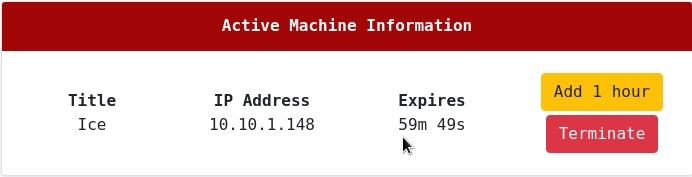
\includegraphics[width=\textwidth]{informacion_maquina.jpeg}
	\caption{Detalles de la maquina}
	\end{figure}
	
	\section{Objetivos}
	Conocer el estado de seguridad actual del servidor \textbf{\machineName}, enumerando
	posibles vectores de explotacion y determinando el alcance e impacto que un atacante
	podria ocasionar sobre el sistema en produccion.
	
	\subsection{Consideraciones}
	Una vez finalizadas las jornadas de auditoria, se llevara a cabo una fase de 
	saneamientos y buenas practicas con el objetivo de securizar el servidor y evitar
	ser victimas de un futuro ataque en base a los vectores explotados. 		

	\vspace{0.5cm}

	\begin{figure}[h]
	\begin{center}
	\smartdiagram[priority descriptive diagram]{
	Reconocimiento sobre el sistema,
	Deteccion de vulnerabilidades,
	Explotacion de vulnerabilidades,
	Securizacion del sistema
	}
	\end{center}
	\caption{Flujo de trabajo}
	\end{figure}

	\clearpage
	\section{Analisis de vulnerabilidades}
	\subsection{Reconocimiento inicial}

	\vspace{0.2cm}
	Se comenzo realizando un analisis inicial sobre el sistema, verificando que el sistema
	objetivo se encontrara accesible desde el segmento de red en el que se opera:

	% foto del ping
	\begin{figure}[h]
	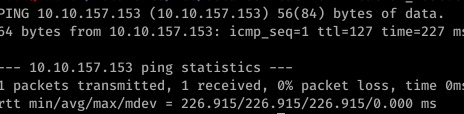
\includegraphics[width=0.8\textwidth]{images/ping_maquina.jpeg}
	\end{figure}

	\vspace{0.2cm}


	\subsection{Reconocimento por Servicios}
	
	Una vez localizado, se realizo un escaneo a traves de la herramienta \textbf{nmap}
	para la deteccion de puertos abiertos.

	% foto del nmap con servicios y scripts basicos
	\begin{figure}[h]
	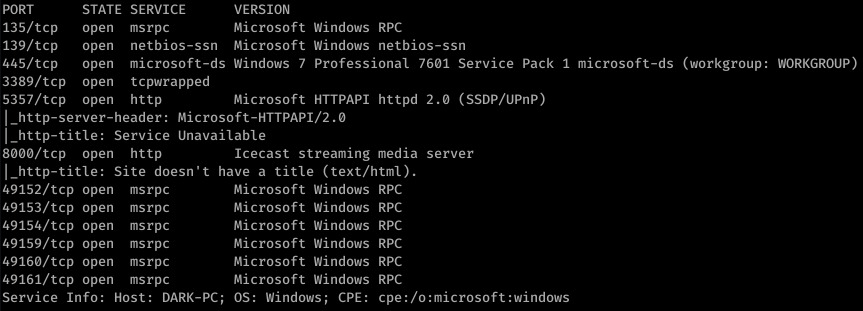
\includegraphics[width=0.8\textwidth]{images/nmap_comun.jpeg}
	\end{figure}

	\subsection{Reconocimento Especifico}
	Al ser uno de los servicios mas usados siempre es conveniente para el atacante mostrar las vulnerabilidades que puede
	o no puede tener este servicio.
	% foto del nmap --script vulns
     \begin{figure}[h]
     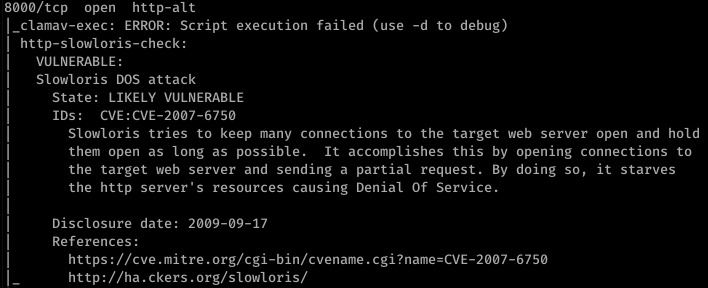
\includegraphics[width=0.8\textwidth]{images/vuln_80.jpeg}
     \end{figure}
	\newpage

	\subsection{Vulnerabilidades}
	Para tener una amplia cantidad de servicios que atacar analizo las vulnerabilidades con el script de la herramienta 
	\textbf{nmap}
	% descripcicion de las vulnerabilidades con lo que 
	% comprete.
      \begin{figure}[h]
      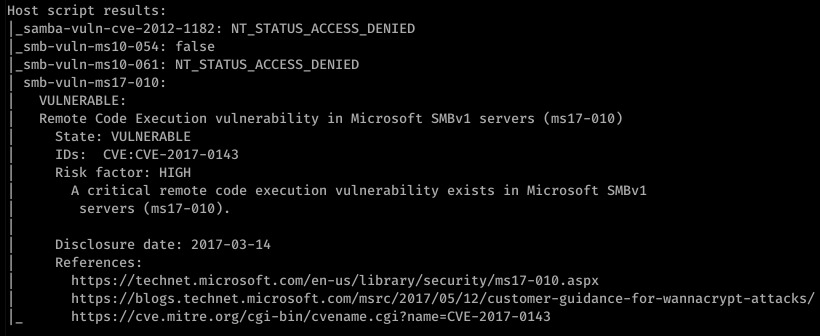
\includegraphics[width=0.8\textwidth]{images/vuln_scripts.jpeg}
      \end{figure}


	\section{Explotacion}

	\subsection{Metodo 1}

	\subsection{Metodo 2}

	\subsection{Metodo 3}

	\section{Post-Explotacion}

	\subsection{Escala de Privilegios}

	\subsection{Persistencia}

	\section{Soluciones}
		
		\subsection{Actividades Post Pentest}

	
\end{document}
